% Copyright (c) 2022 Tobias Briones. All rights reserved.
%
% SPDX-License-Identifier: CC-BY-4.0
%
% This file is part of Course Project at UNAH-IS911: Microprocessors.
%
% This source code is licensed under the Creative Commons Attribution 4.0 
% International License found in the LICENSE file in the root directory of 
% this source tree or at https://spdx.org/licenses/CC-BY-4.0.html.

\documentclass[conference]{IEEEtran}
\usepackage[letterpaper, portrait, margin=2cm]{geometry}
\usepackage[style=ieee]{biblatex}
\usepackage[utf8]{inputenc}
\usepackage[spanish]{babel}
\usepackage{geometry}
\usepackage[]{graphics}
\usepackage[demo]{graphicx}
\usepackage{csquotes}
\usepackage{float}
\usepackage{hyperref}
\usepackage[table,xcdraw]{xcolor}

\addbibresource{bibliography.bib}

\title{SOCKETS DE MICROPROCESADORES DE PC MODERNOS}
\author{

\includegraphics[width = 40mm]{images/logo-unah.png}\\[8ex]
\IEEEauthorblockN{Tobias Briones}
\IEEEauthorblockN{tobias.briones@unah.hn}
\IEEEauthorblockA{\textit{Universidad Nacional Autónoma de Honduras} \\
\textit{Ingeniería de Sistemas} \\
\textit{I PAC 2022} \\
\textit{IS911-MICROPROCESADORES}} \\\vspace*{20pt} \normalsize  \\
\today
}

\hypersetup{
    colorlinks=true,
    linkcolor=black,
    filecolor=magenta,      
    urlcolor=cyan,
    citecolor=black
}
    
\begin{document}

\maketitle

\begin{abstract}
En esta investigación se provee un resumen sobre los sockets para PC modernos año 2022.
\end{abstract}

\tableofcontents

\section{Introducción}

Los sockets son conectores que permiten la conectividad física y eléctrica del microprocesador a la tarjeta madre. Se le denominará a los sockets o slots como zócalos ya que esa es su equivalencia en el español.

\bigbreak

Como se mencionó arriba, podemos afirmar sobre los zócalos el siguiente enunciado:

\begin{displayquote}
    Un zócalo de CPU contiene uno o más componentes mecánicos que proporcionan conexiones mecánicas y eléctricas entre un microprocesador y una placa de circuito impreso (PCB). Esto permite colocar y reemplazar la unidad central de procesamiento (CPU) sin soldar.\\
    \small Fuente: Wikipedia $\mid$ CPU socket \cite{wikipedia-contributors-2022}
\end{displayquote}

\bigbreak

Algunos tipos de sockets, por mencionar, tenemos \cite{authortechnews-2020}: TR4, AM4, LGA 1151, 2066, sTRX4. Al momento de diseñar una configuración para un PC se debe tener en cuenta que la tarjeta madre sea compatible con el resto del hardware escogido y en particular, el socket sea el que corresponde al modelo del CPU que se deberá instalar.

\subsection{Definición}

Una definición simple de un socket es:

\begin{displayquote}
    El \textbf{socket/slot de CPU} o \textbf{zócalo de CPU} se refiere a un conector físico en la placa base de una computadora que acepta un solo chip físico. Muchas placas base pueden tener varios sockets que, a su vez, pueden aceptar chips de varios núcleos.\\
    \small Fuente: University Information Technology Services \cite{university-information-technology-services-2019}
\end{displayquote}

Los ordenadores personales (incluyendo PCs gaming) e industriales cuentan con sockets similares o iguales. Los sockets son mayormente encontrados en estos equipos a diferencia de dispositivos móviles como portátiles o teléfonos inteligentes los cuales traen el CPU soldado en la tarjeta madre o cuentan con un SoC (System on a Chip) el cual es un integrado que implementa el CPU, memoria y demás componentes en un solo chip.

\begin{figure}[H]
    \centering
    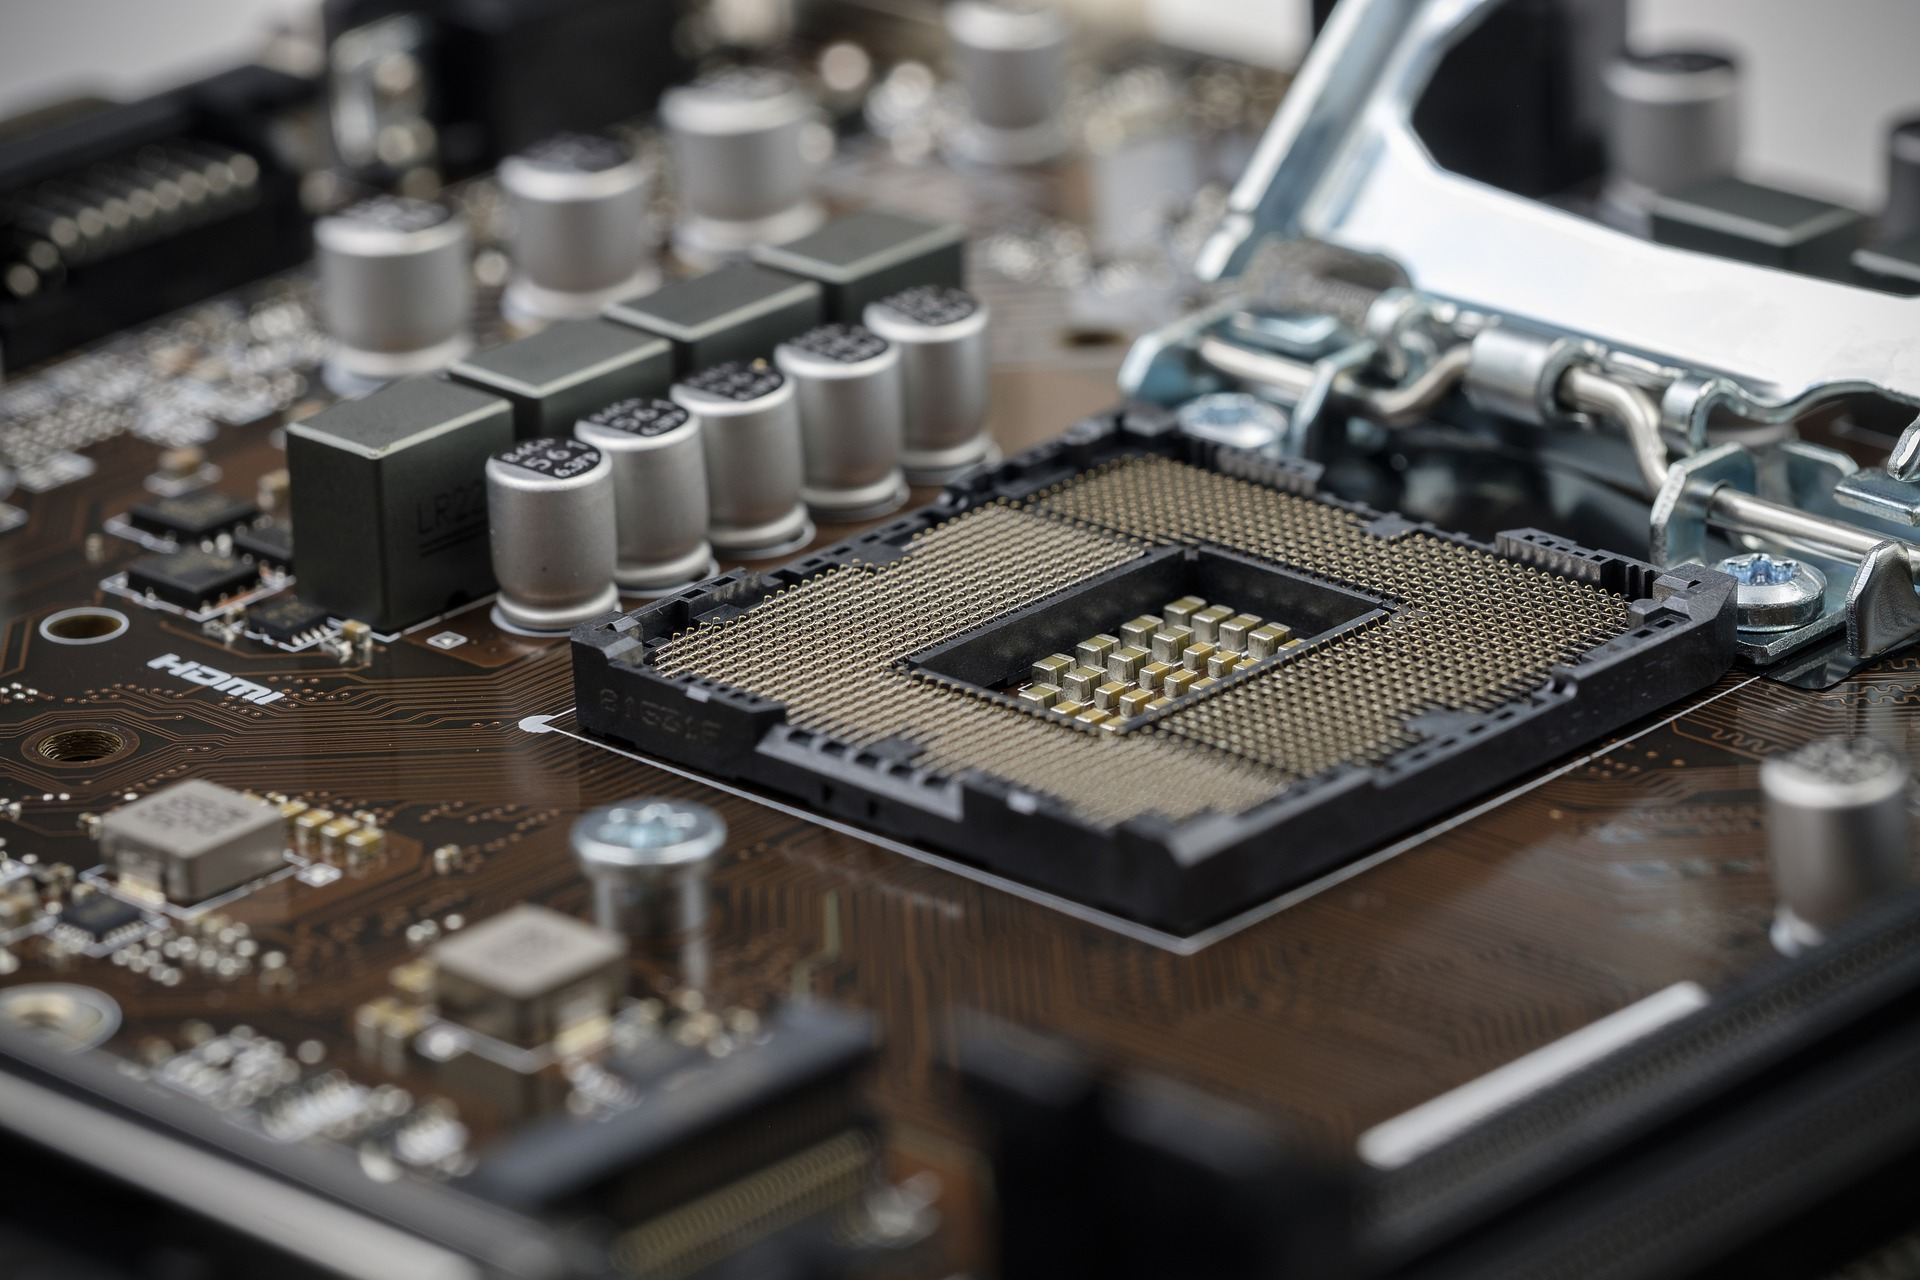
\includegraphics[width=0.3\paperwidth]{images/cpu-socket.jpg}
    \caption{Zócalo de CPU} \footnotesize
    Fuente: Imágen por \href{https://pixabay.com/users/bru-no-1161770}{Bruno /Germany} de \href{https://pixabay.com}{Pixabay} \cite{pixabay-cpu-socket-2019}.
\end{figure}

\section{Tipos de Zócalos}

De acuerdo a datos actuales, se van a presentar los tipos de zócalos que se utilizan en la actualidad para computadoras personales, gaming e incluso también workstation o industriales/servidores.

\bigbreak

Existe una gran cantidad de zócalos viejos \footnote{Wikipedia \cite{wikipedia-contributors-2022} enlista una gran cantidad de modelos incluyendo los viejos introducidos desde el año $1,970$. Si el lector es suficientemente viejo podrá reconocer algunos modelos como el $LGA 775$ en el cual funcionaba nuestros viejos Intel Pentium 4/D o Core2Duo.}, se detallarán solo los más recientes.

\bigbreak

Para escritorio PC se encuentran los siguientes modelos:

\begin{table}[H]
\centering
\tiny
\begin{tabular}{|l|l|l|l|l|}
\hline
\rowcolor[HTML]{CBCEFB} 
\textbf{\begin{tabular}[c]{@{}l@{}}Nombre de \\ Zócalo\end{tabular}} & \textbf{\begin{tabular}[c]{@{}l@{}}Año de \\ Introducción\end{tabular}} & \textbf{CPUs}                                                                                              & \textbf{Paquete} & \textbf{Pines} \\ \hline
Socket AM5                                                           & 2022                                                                    & AMD Zen 4                                                                                                  & LGA              & 1718           \\ \hline
\rowcolor[HTML]{EFEFEF} 
LGA 1700                                                             & 2021                                                                    & Intel Alder Lake                                                                                           & LGA              & 1700           \\ \hline
LGA 1200                                                             & 2020                                                                    & \begin{tabular}[c]{@{}l@{}}Intel Comet Lake\\ Intel Rocket Lake\end{tabular}                               & LGA              & 1200           \\ \hline
\rowcolor[HTML]{EFEFEF} 
\begin{tabular}[c]{@{}l@{}}Socket sTRX4/\\ Socket SP3r3\end{tabular} & 2019                                                                    & \begin{tabular}[c]{@{}l@{}}AMD Ryzen \\ Threadripper\\ (series 3,000)\end{tabular}                         & LGA              & 4094           \\ \hline
\begin{tabular}[c]{@{}l@{}}LGA 2066/Socket\\ R4\end{tabular}         & 2017                                                                    & \begin{tabular}[c]{@{}l@{}}Intel Skylake-X\\ Intel Kaby Lake-X\\ Intel Cascade Lake-X\end{tabular}         & LGA              & 2066           \\ \hline
\rowcolor[HTML]{EFEFEF} 
\begin{tabular}[c]{@{}l@{}}Socket TR4/\\ Socket SP3r2\end{tabular}   & 2017                                                                    & \begin{tabular}[c]{@{}l@{}}AMD Ryzen \\ Threadripper\end{tabular}                                          & LGA              & 4094           \\ \hline
Socket AM4                                                           & 2017                                                                    & \begin{tabular}[c]{@{}l@{}}AMD Ryzen 9\\ AMD Ryzen 7\\ AMD Ryzen 5\\ AMD Ryzen 3\\ Athlon 200\end{tabular} & PGA              & 1331           \\ \hline
\end{tabular}
\caption{Zócalos de CPU recientes}
\small
Fuente: Wikipedia \cite{wikipedia-contributors-2022}.
\end{table}

Los ordenadores se pueden clasificar en convencionales (PC o computador personal), HEDT (High-End Desktop son PC de alto rendimiento), o Servidores/Industriales/Estación de Trabajo. Los zócalos que se listaron son para PCs convencionales de escritorio con CPUs muy populares y algunos de alto rendimiento como los AMD Ryzen™ Threadripper™. Los Intel® Core™ X (LGA 2066/Socket R4) son un ejemplo de modelos para escritorio y para servidor también.

\bigbreak

Entre los modelos mencionados arriba y otros populares se resume la siguiente información más práctica que muestra el modelo de CPU(s), generación, chipsets compatibles y tipo de ordenador personal:

\bigbreak

\begin{itemize}
    \item \textbf{Intel LGA 2066:} 10ma Gen., X299, HEDT.
    \item \textbf{Intel LGA 1200:} 11/10ma Gen., Z490/H470, B460, H410, Convencional.
    \item \textbf{Intel LGA 1151:} 9/8va Gen., Z390/Z370/Z370/Q370/H370/B365/B360/H310, Convencional.
    \item \textbf{AMD sTRX4:} Ryzen Threadripper 3000, TRX40, HEDT.
    \item \textbf{AMD TR4:} Ryzen Threadripper 2000 y 1000, x399, HEDT.
    \item \textbf{AMD AM4:} Ryzen 5000, 3000, 2000 y 1000, X570/X470/X370/B550/B450/B350/B450/A320/X300/A300, Convencional.
\end{itemize}

\small Fuente: tom'sHARDWARE \cite{harding-2021}.

\section{Conclusión}

\printbibliography

\end{document}
